%space 1
%space 2 I hate this box on the top right corner
Projekt byl rozdělen do dvou samostatných častí, které byly vyvíjeny paralelně. První částí je Android aplikace. Druhou částí, která je předmětem této bakalářské práce, je serverový backend, poskytující RESTové služby pro Android aplikace.

Cílem této práce bylo navržení vhodných úprav a následná implementace existujícího návrhu a fragmentů implementace. Také zhodnocení použitelnosti výsledné implementace a navržení vhodných budoucích kroků pro pokračování vývoje serveru. Při implementaci byl také uvažován současný stav souběžně vyvíjené, frontendové části aplikace.

I~když se autor této práce zúčastnil předmětů, během kterých byl udělán předchozí návrh aplikace a fragmenty implementace, byla potřeba přezkoumat návrh programu za účelem vylepšení návrhu a eliminování nalezených nedostatků během implementace frontendové a backendové části. Předchozí implementace programu pokrývala jenom malou část aplikace, proto skoro celá již existující implementace byla přepsána. Byl opraven doménový model, provedeny změny použité třívrstvé architektury, rozšířené API, rozšířená dokumentace API, přidán proces registrace a přihlašování uživatele a také byla implementována bezpečnost aplikace. Při implementaci byly uvazovány požadavky kolegy, který souběžně vyvíjí frontendovou část aplikace.

% Práce se začíná analýzou existujícího návrhu a fragmentů implementace. I když jsem zúčastnil předmětů, které se zabývali těmto návrhem a implementací, potřeboval jsem přezkoumat celý návrh za účelem eliminování, nalezených během implementace frontendové a backendové častí, nedostatků a navržení lepších řešení.
% Potom jsem návrh novou verzí řešení, která obsahuje úpravy podle požadavků frontendové části aplikace a zároveň obsahuje navržené mnou úpravy. Implementace navrženého řešení byla nejsložitější častí této bakalářské práci, protože jsem neměl zkušeností ve vývoje projektů porovnatelného rozsahu a potřeboval jsem naučit mnoha novým věcem.
Důležitou částí této práce bylo testování, které je v~rozsahu napsaného kódu porovnatelné s~implementací serveru samotného. Testy byly rozděleny do dvou typů: unit testy a integrační testy. Unit testy testují samostatně testovatelné funkce programu. Integrační testy využívají za běhu celý kontext aplikace a testují, jestli jednotlivé řadiče fungují správně. 
% \begin{figure}\centering
% 	   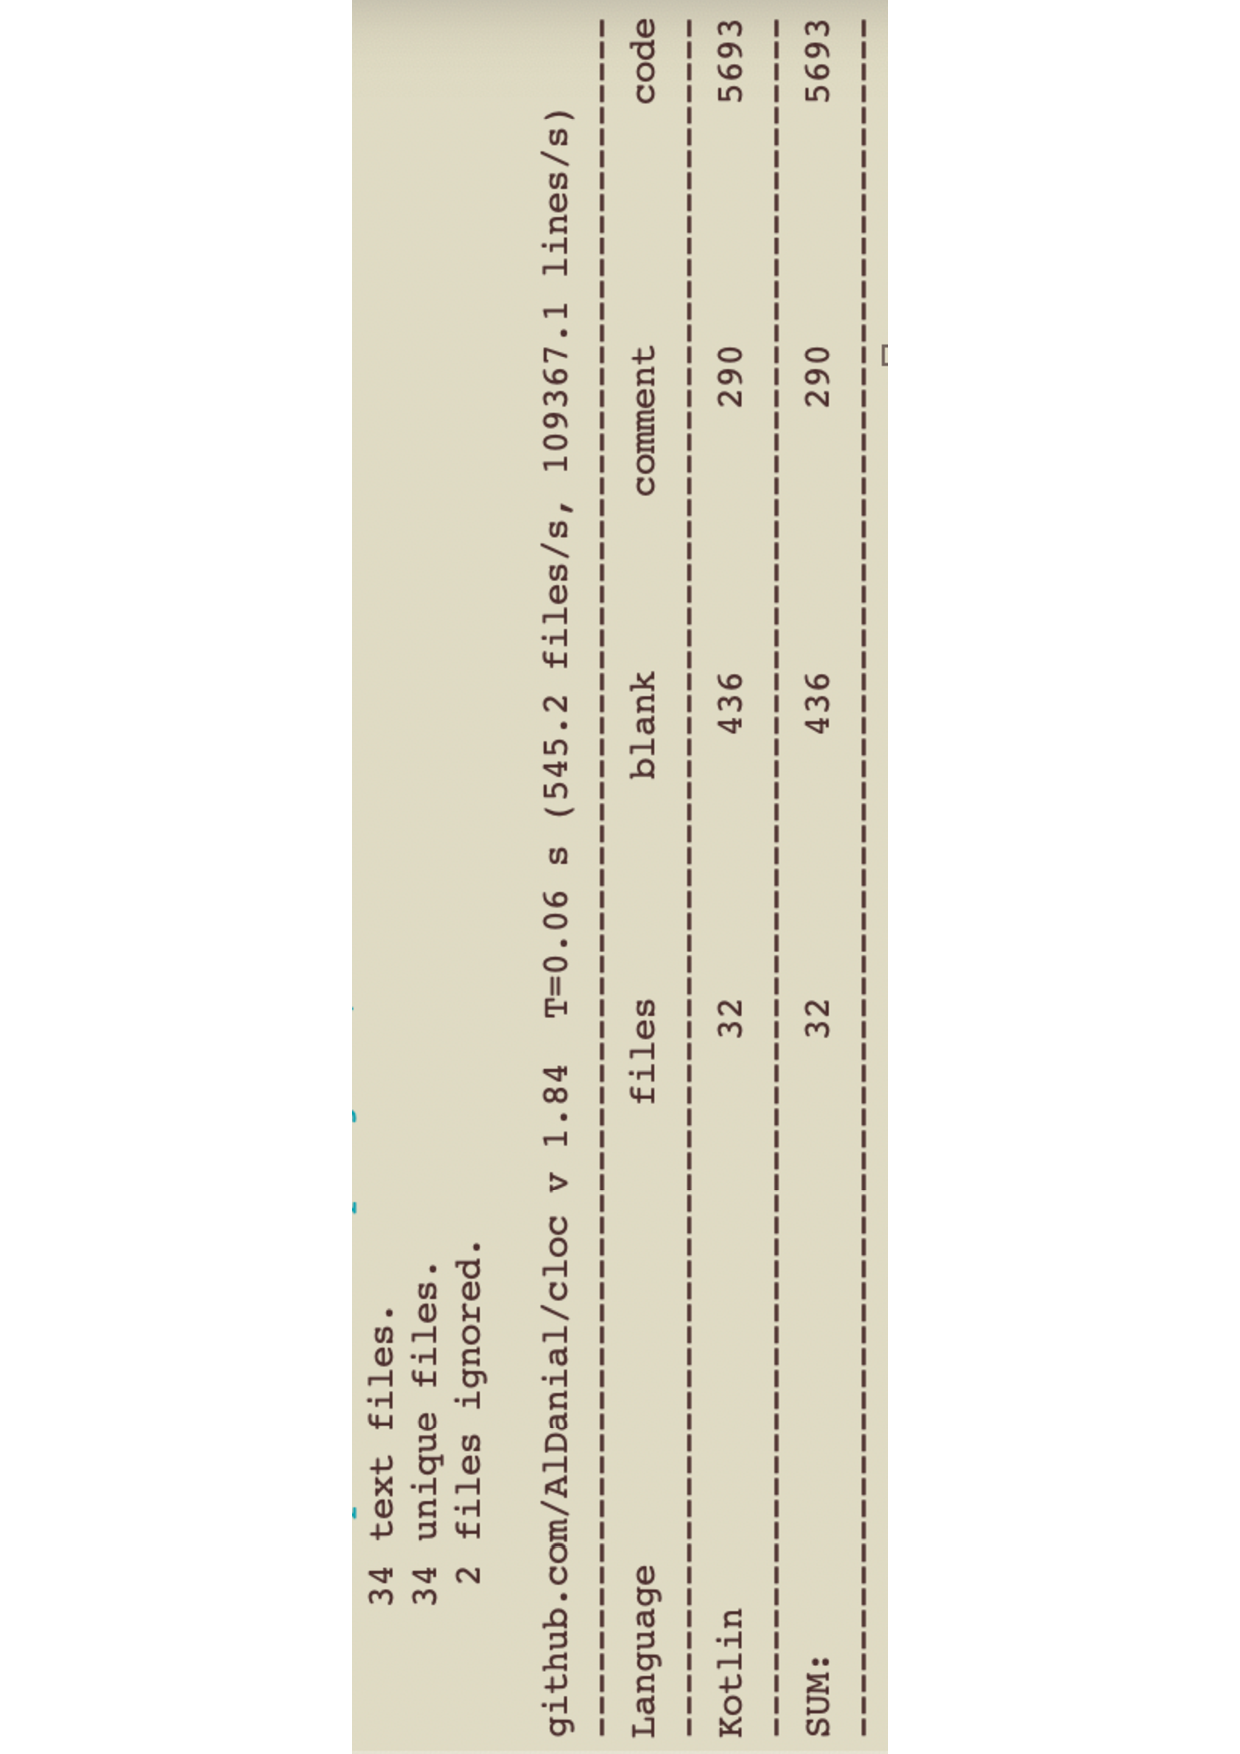
\includegraphics[angle=-90, width=0.5\textwidth]{pdfs/CodeAmountTests2}
% 	   \caption[Analýza kódu testů]{Počet napsáných řádek kódu testů}\label{image:code-count-test}
% \end{figure}
% \begin{figure}\centering
% 	   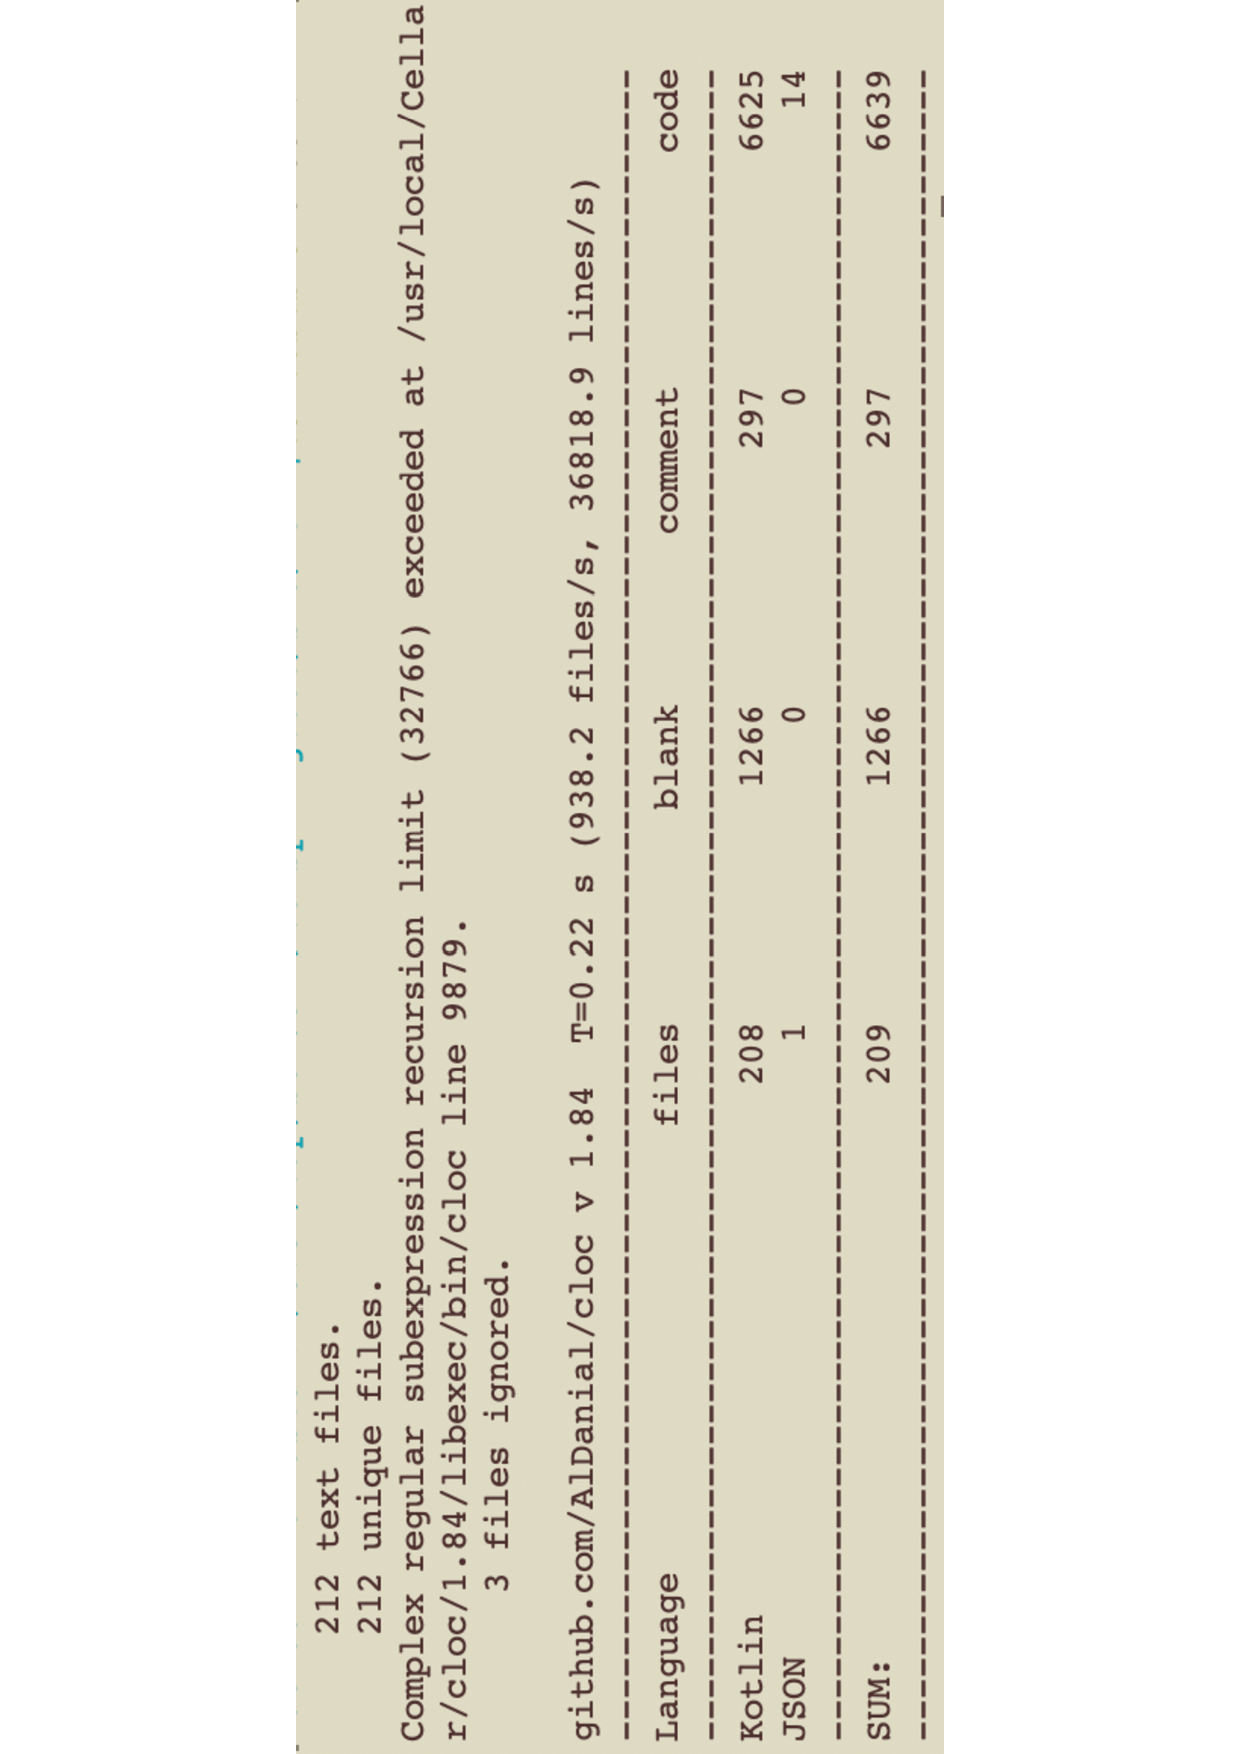
\includegraphics[angle=-90, width=0.5\textwidth]{pdfs/CodeAmountImpl2}
% 	   \caption[Analýza kódu implementace]{Počet napsáných řádek kódu za účelem implementace funkcionality}\label{image:code-count-main}
% \end{figure}

Výsledkem této bakalářské práce je funkční aplikace splňující všechny požadavky frontendové části aplikace. Ale, jak Android aplikace, tak i serverový backend ještě nejsou ve svém finálním stavu. V~rámci této práce byl zhodnocen současný stav a představeny vhodné budoucí kroky pro pokračování vývoje.
% Následující kapitola se věnuje zhodnocení použitelností výsledné implementace a navržení budoucích kroků. Výsledek ještě není připravený pro produkční prostředí a ještě ho očekává dostatečný počet vylepšení. V rámci této bakalářské práci jsem implementoval základ backendu, který má skoro celou potřebnou funkcionalitu, kromě některých věcí, které byly objevený už během pečlivého zanoření do implementace a za
% řazené do budoucích kroků.